\documentclass{article}

\usepackage[nonatbib, final]{neurips_2019}
\usepackage[utf8]{inputenc} % allow utf-8 input
\usepackage[T1]{fontenc}    % use 8-bit T1 fonts
\usepackage{hyperref}       % hyperlinks
\usepackage{url}            % simple URL typesetting
\usepackage{booktabs}       % professional-quality tables
\usepackage{amsfonts}       % blackboard math symbols
\usepackage{nicefrac}       % compact symbols for 1/2, etc.
\usepackage{microtype}      % microtypography
\usepackage{listings}
\usepackage{graphicx}
\usepackage{amsmath}
\usepackage{color}
\usepackage{subfig}         % two images side-by-side
\usepackage{wrapfig, floatrow} % Multipart figures
\usepackage[font=small]{caption}
\usepackage{float}
\usepackage{afterpage}
\usepackage{lipsum}
\hypersetup{
  colorlinks = true, %Colours links
  urlcolor   = blue, %Colour for external hyperlinks
  linkcolor  = blue, %Colour of internal links
  citecolor  = black %Colour of citations
}

\newcommand{\figwithsidecaption}[2]{
\begin{figure}[H]
\floatbox[{\capbeside\thisfloatsetup{capbesideposition={right,top}, capbesidewidth=0.7\textwidth}}]{figure}[\FBwidth]
{\caption*{#1}}
{\includegraphics[width=2cm]{#2}}
\end{figure}
\vspace{-.5cm}
}

\begin{document}

%----------------------------------------------------------------------------------------
%	TITLE PAGE
%----------------------------------------------------------------------------------------

\begin{titlepage} % Suppresses displaying the page number on the title page and the subsequent page counts as page 1
    \newcommand{\HRule}{\rule{\linewidth}{0.5mm}} % Defines a new command for horizontal lines, change thickness here
    

    \center % Centre everything on the page
    
    %------------------------------------------------
    %   Headings
    %------------------------------------------------
    
    \textsc{\LARGE University Of Calgary}\\[1.5cm] % Main heading such as the name of your university/college
    
    \textsc{\Large ENEL 300}\\[0.5cm] % Major heading such as course name
    
    \textsc{\large Electrical Engineering Design}\\[0.5cm] % Minor heading such as course title
    
    %------------------------------------------------
    %   Title
    %------------------------------------------------
    \HRule\\[0.4cm]
    
    {\huge\bfseries Final Technical Report}\\[0.4cm] % Title of your document
    
    \HRule\\[1.5cm]
    
    %------------------------------------------------
    %   Author(s)
    %------------------------------------------------
    \begin{minipage}{0.4\textwidth}
        \begin{flushleft}
            \large
            \textit{Author}\\
            First Author  \\ % Author 1
            Second Author \\ % Author 2
            Third Author  \\ % Author 3
            Fourth Author    % Author 4
        \end{flushleft}
    \end{minipage}
    ~
    \begin{minipage}{0.4\textwidth}
        \begin{flushright}
            \large
            \textit{Course Instructor}\\
            Dr. Laleh \textsc{Behjat} % Supervisor's name
        \end{flushright}
    \end{minipage}
    
    %------------------------------------------------
    %   Date
    %------------------------------------------------
    
    \vfill\vfill\vfill % Position the date 3/4 down the remaining page
    
    {\large \today} % Date, change the \today to a set date if you want to be precise
    
    %------------------------------------------------
    %   Logo
    %------------------------------------------------
    
    \vfill\vfill
    
\includegraphics[width=0.4\textwidth]{./uc-logo.jpg}\\[1cm] % Include a department/university logo - this will require the graphicx package
     
    %----------------------------------------------------------------------------------------
    
    \vfill % Push the date up 1/4 of the remaining page
    
\end{titlepage}
%============================================================================================
\section{Introduction}
\lipsum[1-4]


%============================================================================================
\section{Problem}
\lipsum[8-10]


%============================================================================================
\section{Our solution}
\subsection{Qube platform description}

\begin{figure}%
    \centering
    \subfloat[]{{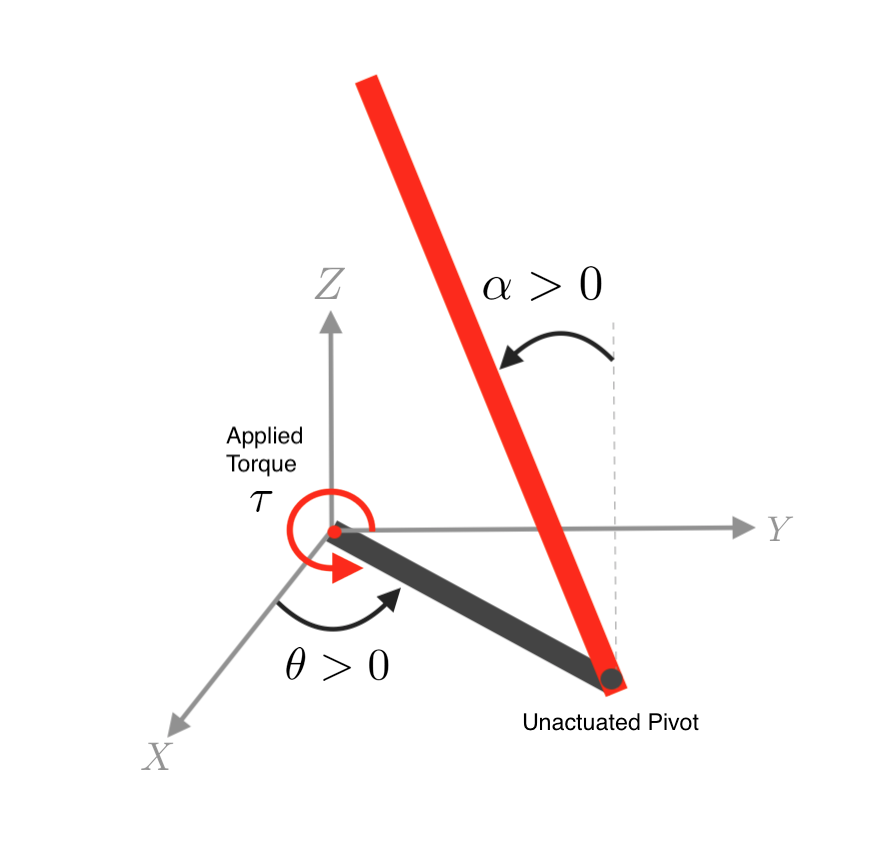
\includegraphics[width=0.25\linewidth]{figures/rotary-pendulum-conventions}}}
    \qquad
    \subfloat[]{{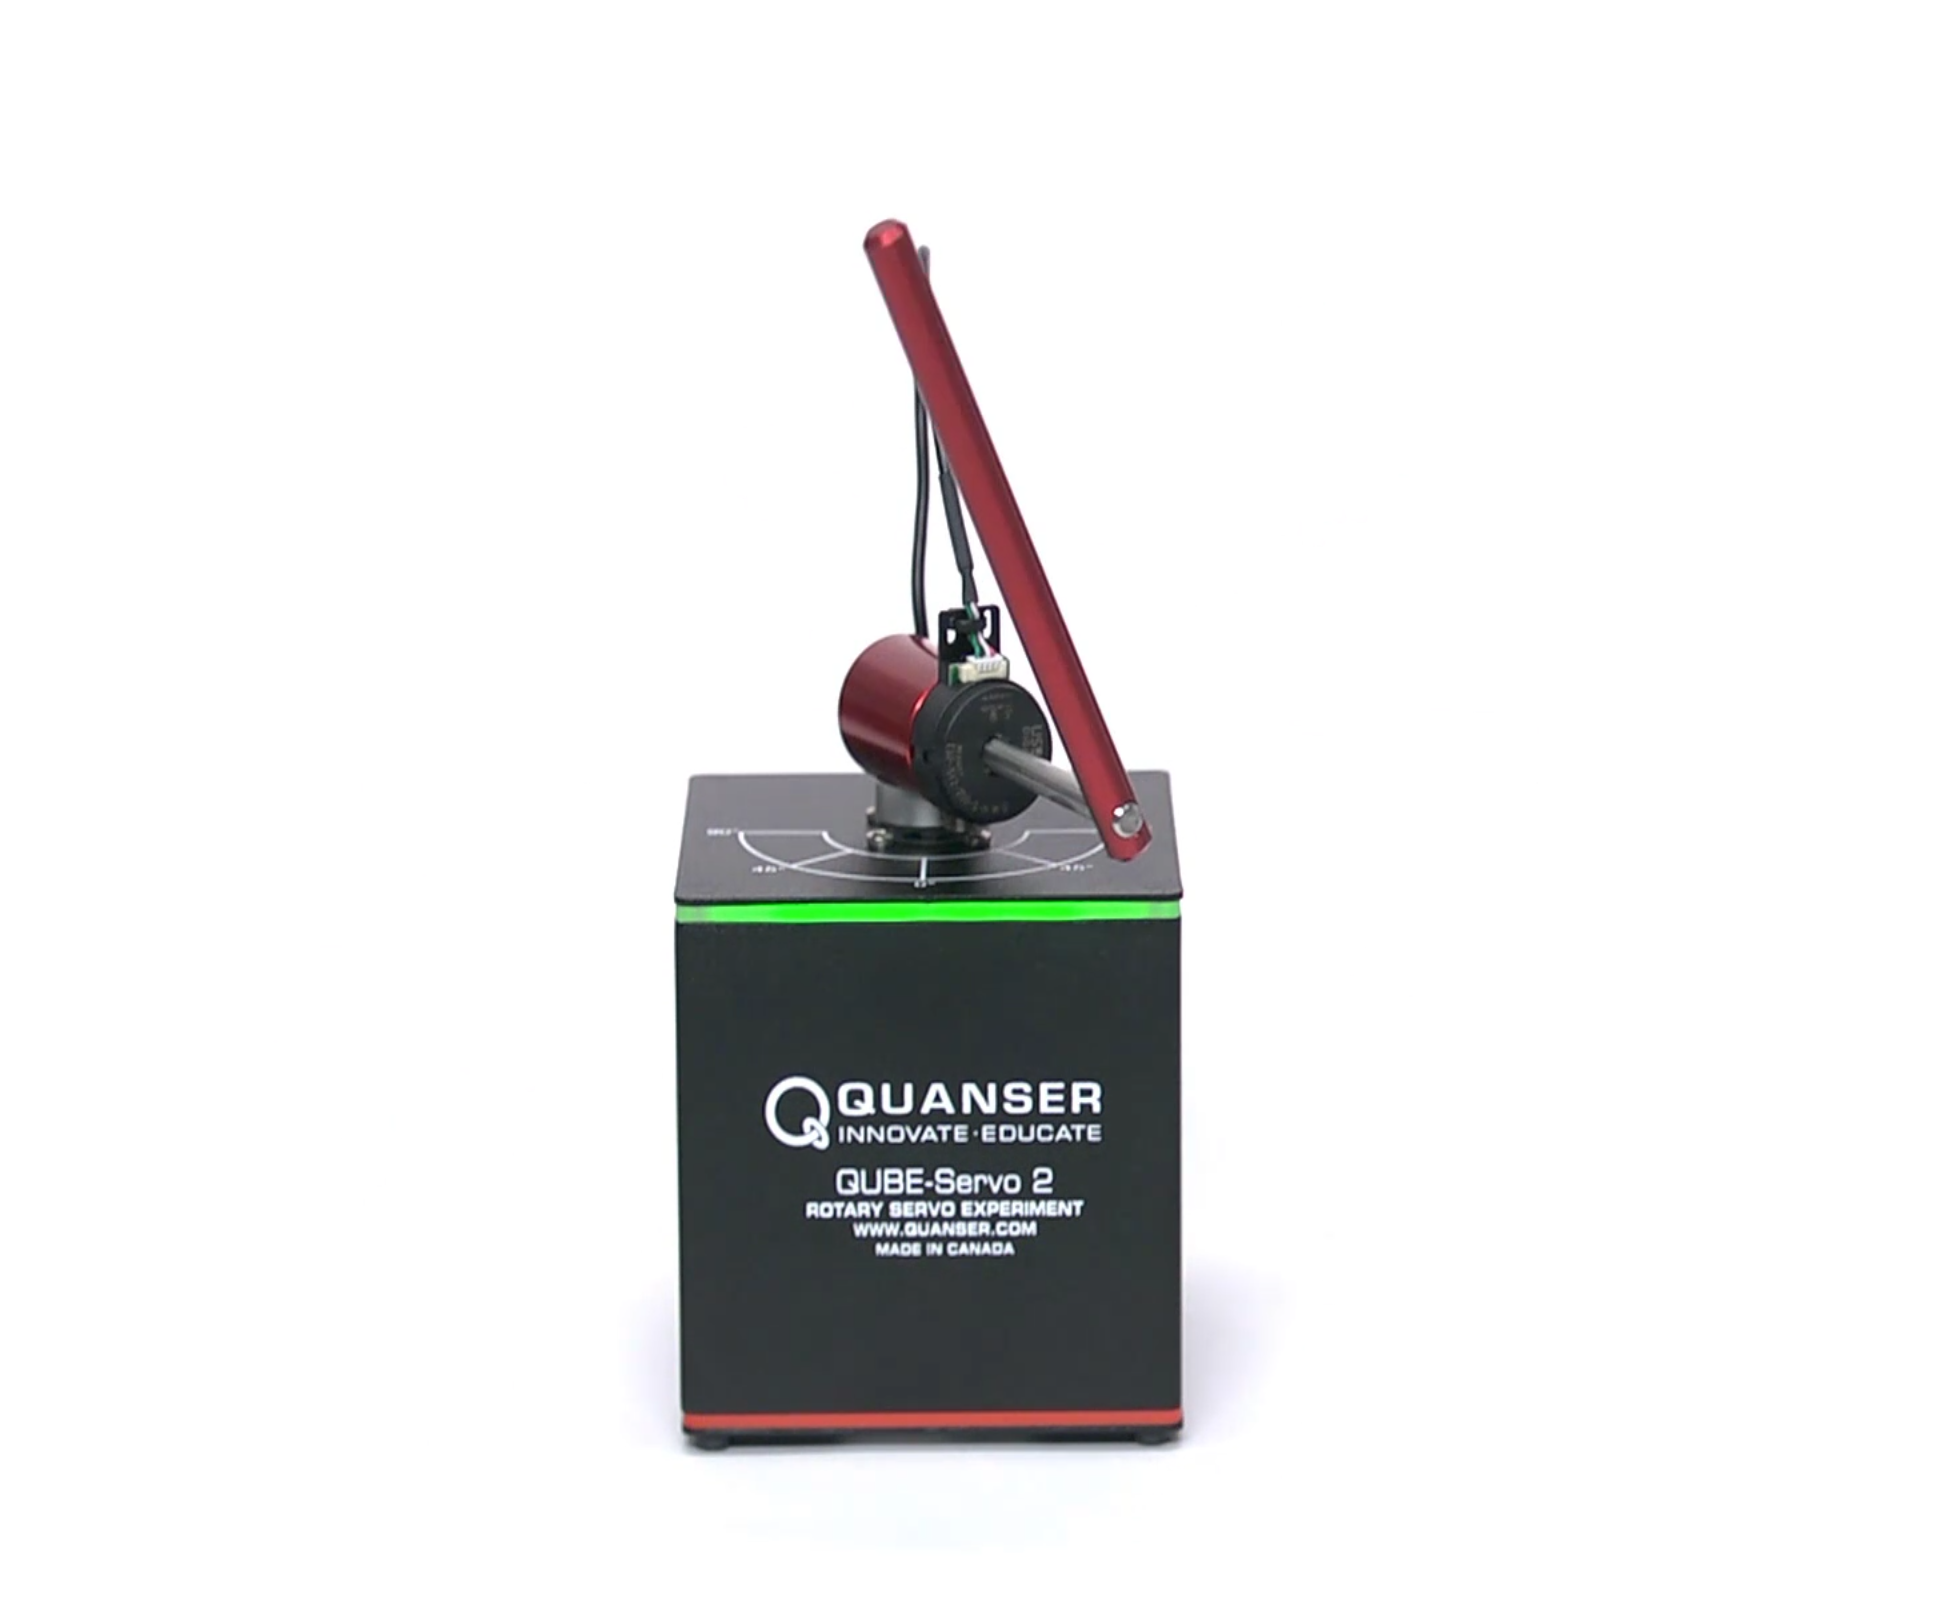
\includegraphics[width=0.3\linewidth]{figures/qube-servo2-usb}}}
    \caption{Qube Servo-2 USB}
    \label{fig:qube-servo2-usb}
\end{figure}

\lipsum[11]

We use the following conventions:
\begin{itemize}
    \item $\alpha$: angle of \emph{pendulum} from upright.
    \item $\theta$: angle of \emph{arm} from centered at the front.
    \item $\dot{\alpha}$: angular velocity of \emph{pendulum} from centered at the front.
    \item $\dot{\theta}$: angular velocity of \emph{arm} from centered at the front.
\end{itemize}


\subsection{RL Gym Tasks for the Qube platform}
\lipsum[12-13]

\figwithsidecaption{\textbf{Dampen}: \lipsum[2]}{figures/dampen}
\figwithsidecaption{\textbf{Balance}: \lipsum[2]}{figures/balance}
\figwithsidecaption{\textbf{Balance Follow}: \lipsum[2]}{figures/balance-follow}
\figwithsidecaption{\textbf{Swing}: \lipsum[2]}{figures/swing}
\figwithsidecaption{\textbf{Swing Follow}: \lipsum[2]}{figures/swing-follow}
\figwithsidecaption{\textbf{Rotor}: \lipsum[2]}{figures/rotor}


%============================================================================================
\section{Reinforcement Learning Interface}

\begin{figure}
    \centering
    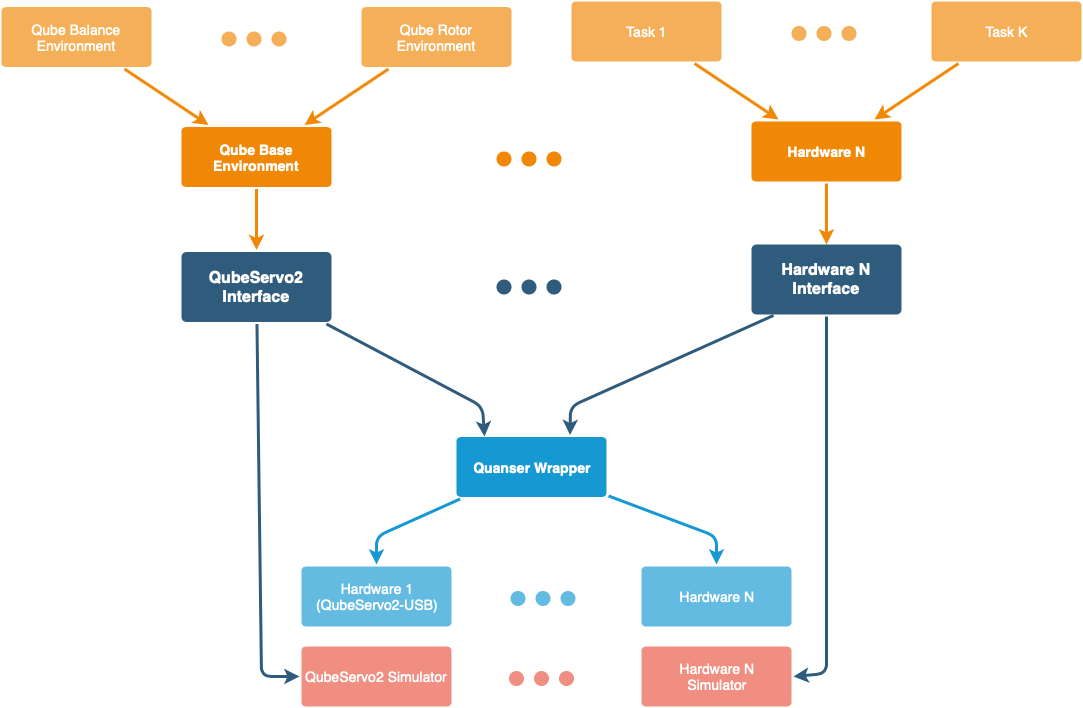
\includegraphics[width=10cm]{figures/high-level-architecture}
    \caption{High level overview of the architecture.}
\end{figure}

\lipsum[15]

\subsection{Base Environment}
\lipsum[19]

\subsection{Reward Debugging}
\lipsum[21]

%============================================================================================
\section{Hardware Interface}

\subsection{Python Wrapper}

\lipsum[22]


A simple example of use with python.

%----- CODE --------------------------------------------------------------------
\begin{verbatim}
from scipy.integrate import odeint
from physics_model import diff_forward_model_ode
import numpy as np


# Motor
Rm, kt, km = 8.4, 0.042, 0.042
# Rotary Arm
mr, Lr, Dr = 0.095, 0.085, 0.00027
# Pendulum Link
mp, Lp, Dp = 0.024,  0.129,  0.00005
g = 9.81
Jr = mr * Lr ** 2 / 12
Jp = mp * Lp ** 2 / 12


def forward_model_ode(theta, alpha, theta_dot, alpha_dot, Vm, dt):
    t = np.linspace(0.0, dt, 2)
    state = np.array([theta, alpha, theta_dot, alpha_dot])
    next_state = odeint(
        diff_forward_model_ode,
        state,
        t,
        args=(Vm, dt)
    )[1, :]
    theta, alpha, theta_dot, alpha_dot = next_state

    theta = ((theta + np.pi) % (2 * np.pi)) - np.pi
    alpha = ((alpha + np.pi) % (2 * np.pi)) - np.pi

    return theta, alpha, theta_dot, alpha_dot
\end{verbatim}
%----- CODE --------------------------------------------------------------------


\lipsum[39]

\subsection{Quanser Interface}
\lipsum[69]

%============================================================================================
\section{Benchmarks}
\lipsum[99]

%============================================================================================
\section{Future Work}
\lipsum[2-3]


\begin{itemize}
\item
    Contact-based physics simulators like Mujoco \cite{mujoco} and Bullet \cite{bullet} add more realism than the physics simulator we currently use.
\item
    Domain randomization has been shown to be a viable method for transfer from simulation to real hardware \cite{Domain-Randomization, Learning-Dexterity}.
\item
    By studying a relatively simple problem like the Qube, it may be easier to observe the effects of different options for accuracy and which portions of simulators to add noise (in the case of domain randomization).
\end{itemize}


\bibliographystyle{unsrt}
\bibliography{main} 

\end{document}
